\documentclass[11pt,letterpaper]{article}
\usepackage[T1]{fontenc}
\usepackage[utf8]{inputenc}
\usepackage{amsmath}
\usepackage{mathptmx}
\usepackage[margin=1in]{geometry}
\usepackage{graphicx}
\usepackage{booktabs}
\usepackage{array}
\usepackage[font={small},labelfont=bf,labelsep=period]{caption}
\usepackage{parskip}
\usepackage{xcolor}
\usepackage[hidelinks]{hyperref}
\usepackage{enumitem}
\setlist{itemsep=2pt,topsep=3pt}
\setlength{\emergencystretch}{2em}
% let figures and tables share pages with text instead of sitting on half-empty float pages
\renewcommand{\topfraction}{0.9}
\renewcommand{\bottomfraction}{0.8}
\renewcommand{\textfraction}{0.07}
\renewcommand{\floatpagefraction}{0.75}
\setcounter{topnumber}{3}
\setcounter{bottomnumber}{2}
\setcounter{totalnumber}{4}
\makeatletter
\setlength{\@fptop}{0pt}
\setlength{\@fpsep}{12pt plus 4pt}
\setlength{\@fpbot}{0pt plus 1fil}
\makeatother
\graphicspath{{../figures/}}
\newcommand{\AblMiddleOnlyLr}{51.6}
\newcommand{\AblMiddleOnlyRetrain}{50.8}
\newcommand{\AblMiddleOnlyTest}{45.4}
\newcommand{\AblNoFormatLr}{53.8}
\newcommand{\AblNoFormatRetrain}{48.1}
\newcommand{\AblNoFormatTest}{32.5}
\newcommand{\AblOpeningOnlyLr}{50.3}
\newcommand{\AblOpeningOnlyRetrain}{46.7}
\newcommand{\AblOpeningOnlyTest}{43.5}
\newcommand{\AblOriginalLr}{63.3}
\newcommand{\AblOriginalRetrain}{63.0}
\newcommand{\AblOriginalTest}{63.0}
\newcommand{\AblSeeds}{3}
\newcommand{\AblStructureOnlyLr}{58.3}
\newcommand{\AblStructureOnlyRetrain}{61.3}
\newcommand{\AblStructureOnlyTest}{48.5}
\newcommand{\AblWordsOnlyLr}{51.9}
\newcommand{\AblWordsOnlyRetrain}{46.6}
\newcommand{\AblWordsOnlyTest}{27.4}
\newcommand{\AgreeAcc}{77.0}
\newcommand{\AgreeRate}{67.2}
\newcommand{\BestRunAcc}{65.2}
\newcommand{\BiasOneCnn}{60.0}
\newcommand{\BiasOneLr}{57.4}
\newcommand{\BiasOneMaj}{30.3}
\newcommand{\BiasZeroCnn}{17.2}
\newcommand{\BiasZeroLr}{19.8}
\newcommand{\CnnAcc}{63.0}
\newcommand{\CnnAccSd}{2.1}
\newcommand{\CnnBestEpochs}{14, 11, 9}
\newcommand{\CnnEpochs}{11}
\newcommand{\CnnFone}{61.9}
\newcommand{\CnnMax}{65.2}
\newcommand{\CnnMin}{60.9}
\newcommand{\CnnMinutes}{6}
\newcommand{\CnnParams}{2,041,402}
\newcommand{\CnnSecEpochHi}{37}
\newcommand{\CnnSecEpochLo}{23}
\newcommand{\CnnSeeds}{3}
\newcommand{\CnnVocab}{14,732}
\newcommand{\CurlyGpt}{22}
\newcommand{\CurlyQwen}{8}
\newcommand{\DashBulletLlama}{0.5}
\newcommand{\DisagreeAcc}{40.8}
\newcommand{\EnsAcc}{67.6}
\newcommand{\EnsGain}{4.4}
\newcommand{\EnsGainRun}{2.5}
\newcommand{\EnsN}{7}
\newcommand{\FeatAllFeatures}{46.0}
\newcommand{\FeatFormattingOnly}{39.2}
\newcommand{\FeatLengthOnly}{28.3}
\newcommand{\FeatLinguisticOnly}{30.6}
\newcommand{\FilterCnnAcc}{65.2}
\newcommand{\LongCnnAcc}{70.3}
\newcommand{\LrAcc}{63.3}
\newcommand{\LstmAcc}{59.6}
\newcommand{\LstmAccSd}{1.6}
\newcommand{\LstmBestEpochs}{12, 14, 13}
\newcommand{\LstmEpochs}{13}
\newcommand{\LstmFone}{58.8}
\newcommand{\LstmMax}{61.5}
\newcommand{\LstmMin}{58.5}
\newcommand{\LstmMinutes}{39}
\newcommand{\LstmParams}{1,986,566}
\newcommand{\LstmSecEpochHi}{179}
\newcommand{\LstmSecEpochLo}{138}
\newcommand{\LstmSeeds}{3}
\newcommand{\LstmVocab}{14,732}
\newcommand{\MedianWords}{232}
\newcommand{\NPrompts}{804}
\newcommand{\NRows}{4,824}
\newcommand{\QaCnnAcc}{68.5}
\newcommand{\QaLrAcc}{65.9}
\newcommand{\RecallCnnClaude}{88.3}
\newcommand{\RecallCnnDeepSeek}{48.1}
\newcommand{\RecallCnnGPT}{51.9}
\newcommand{\RecallCnnGemini}{72.4}
\newcommand{\RecallCnnLlama}{82.2}
\newcommand{\RecallCnnQwen}{35.0}
\newcommand{\RecallCrossCodingClaude}{79}
\newcommand{\RecallCrossCodingDeepSeek}{29}
\newcommand{\RecallCrossCodingGPT}{48}
\newcommand{\RecallCrossCodingGemini}{48}
\newcommand{\RecallCrossCodingLlama}{56}
\newcommand{\RecallCrossCodingQwen}{30}
\newcommand{\RecallCrossWritingClaude}{62}
\newcommand{\RecallCrossWritingDeepSeek}{41}
\newcommand{\RecallCrossWritingGPT}{31}
\newcommand{\RecallCrossWritingGemini}{41}
\newcommand{\RecallCrossWritingLlama}{60}
\newcommand{\RecallCrossWritingQwen}{45}
\newcommand{\RecallCtrlCodingClaude}{79}
\newcommand{\RecallCtrlCodingDeepSeek}{37}
\newcommand{\RecallCtrlCodingGPT}{51}
\newcommand{\RecallCtrlCodingGemini}{61}
\newcommand{\RecallCtrlCodingLlama}{58}
\newcommand{\RecallCtrlCodingQwen}{22}
\newcommand{\RecallCtrlWritingClaude}{71}
\newcommand{\RecallCtrlWritingDeepSeek}{39}
\newcommand{\RecallCtrlWritingGPT}{28}
\newcommand{\RecallCtrlWritingGemini}{55}
\newcommand{\RecallCtrlWritingLlama}{65}
\newcommand{\RecallCtrlWritingQwen}{35}
\newcommand{\RowSplitGap}{16}
\newcommand{\RowSplitLr}{47.3}
\newcommand{\RqOneGap}{3}
\newcommand{\RqThreeCodingCnnCiHi}{5.8}
\newcommand{\RqThreeCodingCnnCiLo}{$-$0.2}
\newcommand{\RqThreeCodingCnnCross}{48.6}
\newcommand{\RqThreeCodingCnnCtrl}{51.4}
\newcommand{\RqThreeCodingCnnDrop}{2.8}
\newcommand{\RqThreeCodingCnnNTarget}{60}
\newcommand{\RqThreeCodingCnnSrc}{67.0}
\newcommand{\RqThreeWritingCnnCiHi}{3.9}
\newcommand{\RqThreeWritingCnnCiLo}{0.9}
\newcommand{\RqThreeWritingCnnCross}{46.6}
\newcommand{\RqThreeWritingCnnCtrl}{49.0}
\newcommand{\RqThreeWritingCnnDrop}{2.4}
\newcommand{\RqThreeWritingCnnNTarget}{162}
\newcommand{\RqThreeWritingCnnSrc}{66.1}
\newcommand{\RqThreeWritingLstmCiHi}{5.2}
\newcommand{\RqThreeWritingLstmCiLo}{$-$0.9}
\newcommand{\RqThreeWritingLstmCross}{40.8}
\newcommand{\RqThreeWritingLstmCtrl}{43.1}
\newcommand{\RqThreeWritingLstmDrop}{2.3}
\newcommand{\RqThreeWritingLstmNTarget}{162}
\newcommand{\RqThreeWritingLstmSrc}{61.5}
\newcommand{\RqTwoInCnn}{16.7}
\newcommand{\RqTwoInLr}{16.7}
\newcommand{\RqTwoInLstm}{16.7}
\newcommand{\RqTwoInOutCnn}{64.7}
\newcommand{\RqTwoInOutLr}{63.3}
\newcommand{\RqTwoInOutLstm}{58.6}
\newcommand{\RqTwoOutCnn}{63.0}
\newcommand{\RqTwoOutLr}{63.3}
\newcommand{\RqTwoOutLstm}{59.6}
\newcommand{\ShareBoldClaude}{0}
\newcommand{\ShareBoldDeepSeek}{1}
\newcommand{\ShareBoldGPT}{61}
\newcommand{\ShareBoldGemini}{48}
\newcommand{\ShareBoldLlama}{64}
\newcommand{\ShareBoldQwen}{32}
\newcommand{\ShareBulletsClaude}{26}
\newcommand{\ShareBulletsDeepSeek}{10}
\newcommand{\ShareBulletsGPT}{41}
\newcommand{\ShareBulletsGemini}{42}
\newcommand{\ShareBulletsLlama}{36}
\newcommand{\ShareBulletsQwen}{18}
\newcommand{\ShareHeadersClaude}{2}
\newcommand{\ShareHeadersDeepSeek}{1}
\newcommand{\ShareHeadersGPT}{30}
\newcommand{\ShareHeadersGemini}{2}
\newcommand{\ShareHeadersLlama}{1}
\newcommand{\ShareHeadersQwen}{9}
\newcommand{\ShareNumberedClaude}{74}
\newcommand{\ShareNumberedDeepSeek}{40}
\newcommand{\ShareNumberedGPT}{56}
\newcommand{\ShareNumberedGemini}{42}
\newcommand{\ShareNumberedLlama}{50}
\newcommand{\ShareNumberedQwen}{46}
\newcommand{\ShareUnderFifty}{8}
\newcommand{\ShareUnderOneFifty}{24}
\newcommand{\ShareUnderOneFiftyClaude}{17}
\newcommand{\ShareUnderOneFiftyDeepSeek}{31}
\newcommand{\ShortCnnAcc}{38.2}
\newcommand{\ShortLrAcc}{45.0}
\newcommand{\ShortN}{131}
\newcommand{\WritingCnnAcc}{46.7}
\newcommand{\WritingLrAcc}{55.2}

\newcommand{\ttt}[1]{\texttt{\small #1}}
\makeatletter\newcommand\tabinput[1]{\@@input #1 }\makeatother
\newcommand{\two}[2]{\begin{tabular}[b]{@{}c@{}}#1\\#2\end{tabular}}

\begin{document}

\begin{center}
{\LARGE\bfseries Who Wrote It? Identifying LLMs from Their Responses\par}
\vspace{6pt}
{\large CMPSC 448 Midterm Project\par}
\vspace{4pt}
{\large Siyi Luo \,(team leader and only member; individual project)\par}
\vspace{4pt}
{\normalsize Code and data: \url{https://github.com/borispie/who-wrote-it-llm-id}\par}
\end{center}

\section{Problem definition}

Chatbots now write a lot of the text we read. In this project I ask a simple question: \emph{if I give a computer
an answer written by a large language model (LLM), can it tell which LLM wrote it?}

I set this up as a classification problem with six classes. Each example has three parts: the name of the LLM,
the user's prompt (the \emph{input}) and the LLM's answer (the \emph{output}). The label is the LLM family: GPT,
Claude, Gemini, Llama, Qwen or DeepSeek. Random guessing would be right 1 time in 6, which is 16.7\%.

In this report, ``LLM'' means the chatbot that wrote an answer, and ``classifier'' means my own model. I call the
habits that make one LLM's answers easy to recognize its \emph{fingerprint}. I trained the two required
classifiers, a CNN and an RNN (a bidirectional LSTM, or ``BiLSTM''), and used them to answer four questions:
\begin{itemize}
  \item \textbf{RQ1.} Can we tell which LLM wrote an answer, using only the answer?
  \item \textbf{RQ2.} Does it help to also show the classifier the prompt?
  \item \textbf{RQ3 (extra credit).} Does the fingerprint still work on a kind of task the classifier never saw?
  \item \textbf{RQ4 (extra credit).} What makes the LLMs different, and what happens if we remove those differences?
\end{itemize}

\section{Dataset curation}

\textbf{Where the data comes from.} I did not collect any chats myself. I used the public answers released with
\textbf{AlpacaEval} \cite{alpacaeval}, a well-known benchmark for chatbots (GitHub \ttt{tatsu-lab/alpaca\_eval},
Apache-2.0 license). For hundreds of models, it stores the model's answers to the same 805 prompts, and each
record already has the three fields I need: model name, prompt and answer. I picked one model per family
(Table~\ref{tab:data}). I chose this source for three reasons:
\begin{enumerate}
  \item It is public and has no private or personal data.
  \item Every model answered the \emph{same} prompts. So the classes are perfectly balanced, and the topic of a
        prompt cannot give away which LLM answered it (this matters for RQ2).
  \item It has all six families I wanted.
\end{enumerate}
My script \ttt{src/build\_dataset.py} downloads the files from one fixed version of the repository (commit
\ttt{cd543a1}), so anyone can rebuild exactly the same dataset.

\begin{table}[!htbp]
\centering
\caption{The six LLMs (one model per family). Every model answered the same \NPrompts{} prompts.}
\label{tab:data}
\small
\begin{tabular}{llrrr}
\toprule
Family & Model (name in AlpacaEval) & Answers & Median words & Mean words \\
\midrule
\tabinput{tables/dataset.tex}
\bottomrule
\end{tabular}
\end{table}

\textbf{Cleaning.} One prompt had an empty answer from one model, so I removed that prompt for all six models.
That leaves \NPrompts{} prompts $\times$ 6 = \NRows{} answers, exactly \NPrompts{} per family. They are saved
in \ttt{data/llm\_responses.csv} with the columns \ttt{llm\_name}, \ttt{llm\_input} and \ttt{llm\_output}, plus
a prompt id, the family, the prompt's source, the task type and the split. I kept every answer
as it was written, including markdown (\ttt{\#}, \ttt{**}, bullet points), line breaks and emojis, because how an
LLM formats its answer is part of its style.

\textbf{Task types (needed for RQ3).} AlpacaEval does not say what kind of task each prompt is, so I labeled the
prompts with simple keyword rules. For example, ``python'' or ``SQL'' means \emph{coding}, ``solve'' means
\emph{math}, and ``poem'' or ``email'' means \emph{writing}; everything else is \emph{QA / advice}. Rules make
mistakes (``Write a script for a YouTube video'' is writing, not coding), so I read all the coding and math prompts
and fixed 38 labels by hand. The final counts are 549 QA / advice, 162 writing, 60 coding and 33 math prompts.

\textbf{Train / validation / test split.} I split the data \textbf{by prompt}: 70\% of the prompts for training
(562), 15\% for validation (120) and 15\% for testing (122). All six answers to one prompt always go to the same
part, so every test prompt is new to the classifier, just like in real use.

\section{Models and training}

\textbf{From text to numbers.} I wrote a small tokenizer that splits the text into words, numbers and punctuation
marks. It also keeps formatting marks as their own tokens: a line break becomes \ttt{<nl>}, and markdown symbols
like \ttt{**} and \ttt{\#} are kept. Words are lowercased. Answers are long (median \MedianWords{} words) and I
only had a CPU, so I kept the \textbf{first 200 and last 50 tokens} of each answer. The vocabulary
(\CnnVocab{} tokens) is built from the training answers only. For RQ2, the prompt (up to 64 tokens) is put in
front of the answer.

\textbf{The two classifiers.} Both start the same way: each token becomes a list of 128 numbers (an
\emph{embedding}) that the model learns during training. Table~\ref{tab:models} lists all settings.
\begin{itemize}
  \item \textbf{CNN} (following Kim \cite{kim2014}). The CNN slides 300 small filters over the text. Each filter
        looks at 3, 4 or 5 tokens at a time and learns to spot one short pattern, such as ``here's a'' or a line
        break followed by \ttt{**}. For each filter, the model keeps only its strongest match anywhere in the
        answer (\emph{max-pooling}). A final layer turns these 300 numbers into 6 scores, one per family.
  \item \textbf{BiLSTM} \cite{lstm}. An LSTM reads the tokens one at a time and keeps a memory of what it has
        read so far. A bidirectional LSTM uses two of them: one reads left to right, the other right to left. I
        take the average and the maximum of its outputs over the whole answer, and a final layer gives 6 scores.
\end{itemize}

\begin{table}[!htbp]
\centering
\caption{Classifier and training settings.}
\label{tab:models}
\small
\begin{tabular}{lll}
\toprule
 & CNN & BiLSTM \\
\midrule
Input & \multicolumn{2}{l}{first 200 + last 50 tokens of the answer} \\
Embedding & \multicolumn{2}{l}{128 numbers per token, learned from scratch (20\% dropout)} \\
Main layer & 300 filters: 100 each of width 3, 4, 5 & 1 BiLSTM layer, 64 units per direction \\
Summary of the answer & strongest match of each filter & average + maximum over all tokens \\
Output & \multicolumn{2}{l}{50\% dropout, then a linear layer with 6 outputs} \\
Parameters & \CnnParams & \LstmParams \\
Time per epoch (1 CPU thread) & \CnnSecEpochLo--\CnnSecEpochHi{} seconds & \LstmSecEpochLo--\LstmSecEpochHi{} seconds \\
\midrule
\multicolumn{3}{l}{\emph{Training (the same for both)}} \\
Loss, optimizer & \multicolumn{2}{l}{cross-entropy; AdamW \cite{adamw} (learning rate 0.001, weight decay 0.0001)} \\
Batch size, epochs & \multicolumn{2}{l}{32; at most 15 epochs; gradient clipping at 1.0} \\
Early stopping & \multicolumn{2}{l}{keep the best epoch (by validation macro-F1); stop after 3 epochs with no gain} \\
Random seeds & \multicolumn{2}{l}{CNN: 3 everywhere. BiLSTM: 3 for RQ1, 1 for the other experiments} \\
\bottomrule
\end{tabular}
\end{table}

\textbf{Training.} Both classifiers are trained the same way. After each pass over the training data (an
\emph{epoch}), I check the score on the validation set and keep the best version of the model. If the score does
not improve for 3 epochs in a row, training stops early. The test set is used only once, at the end. Results
change a little with the random seed, so I trained each CNN setting 3 times and report the average $\pm$
standard deviation. The BiLSTM is about 5 times slower, so it got 3 seeds for RQ1 and 1 seed for the other
experiments. Everything ran in PyTorch on a CPU with 2 cores and no GPU.

\textbf{Baselines and metrics.} To know whether the neural classifiers are any good, I compare them with random
guessing (16.7\%) and with a simple classic model, \textbf{TF-IDF + logistic regression}. It counts which words
and word pairs appear in an answer and learns one weight for each. I report \textbf{accuracy} (the share of
answers labeled correctly) and \textbf{macro-F1}, the average F1 score over the six families. A family's F1 is
high only if the classifier finds most of that family's answers \emph{and} is usually right when it guesses that
family.

\section{Results}

\subsection{RQ1: Can we tell which LLM wrote an answer?}

\textbf{Yes, much better than guessing.} Using only the answer, the CNN picks the right LLM \CnnAcc\% of the time
and the BiLSTM \LstmAcc\% of the time (Table~\ref{tab:rq1}). Guessing gets 16.7\%, so both are about 3.5 to 4
times better.

The CNN is about \RqOneGap{} points ahead of the BiLSTM, but their results over the 3 seeds overlap (CNN
\CnnMin--\CnnMax\%, BiLSTM \LstmMin--\LstmMax\%), so I cannot say the CNN is clearly better. The simple TF-IDF
baseline (\LrAcc\%) does as well as the CNN. This suggests that most of the fingerprint is in \emph{which} words,
short phrases and formatting marks appear. Word counts, or a CNN with short filters, can catch that easily. Reading
the whole answer in order, like the BiLSTM does, does not add much here.

\begin{table}[!htbp]
\centering
\caption{RQ1 test results using only the answer. CNN and BiLSTM: average $\pm$ standard deviation over 3 seeds.
The last six columns are the F1 score (\%) for each family.}
\label{tab:rq1}
\small\setlength{\tabcolsep}{4.5pt}
\begin{tabular}{lcccccccc}
\toprule
Classifier & Accuracy (\%) & Macro-F1 (\%) & GPT & Claude & Gemini & Llama & Qwen & DeepSeek \\
\midrule
\tabinput{tables/rq1.tex}
\bottomrule
\end{tabular}
\end{table}

\begin{figure}[!htbp]
\centering
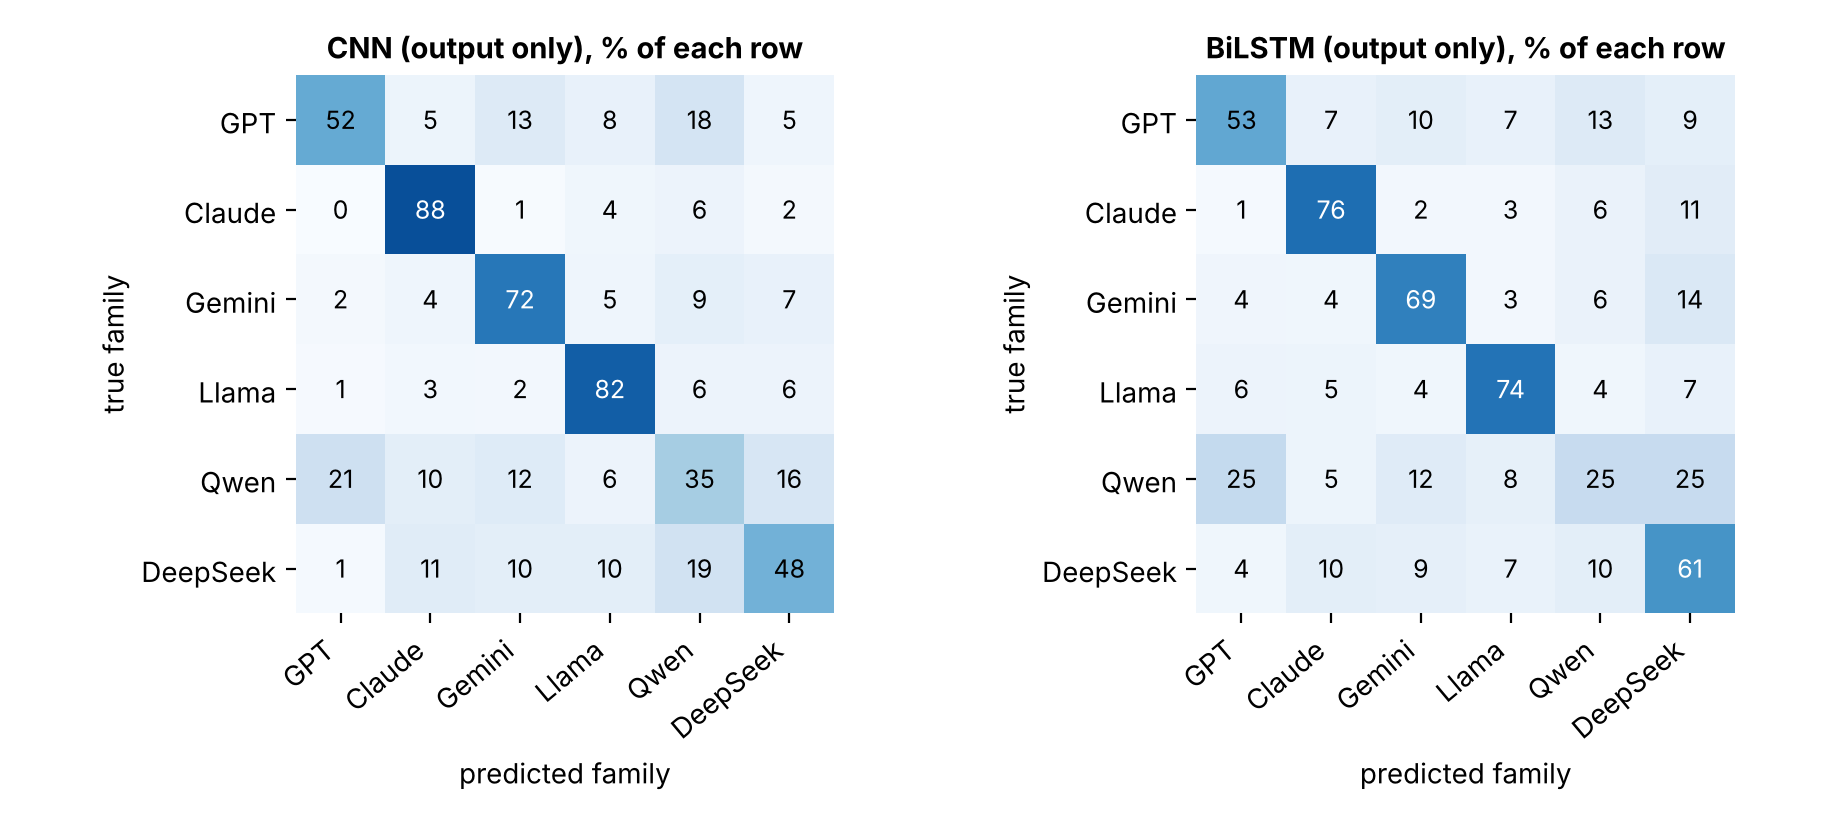
\includegraphics[width=0.98\linewidth]{fig_confusion.png}
\caption{Confusion matrices on the test set (3 seeds together). Each row is the true LLM and shows where its
answers went (\% of the row). The diagonal is the share of that LLM's answers that were labeled correctly.}
\label{fig:cm}
\end{figure}

\textbf{Some LLMs are much easier to spot than others} (Figure~\ref{fig:cm}). Claude and Llama are the easiest:
the CNN finds \RecallCnnClaude\% of Claude's answers and \RecallCnnLlama\% of Llama's. Qwen is the hardest
(\RecallCnnQwen\%) and is often mistaken for GPT or DeepSeek. RQ4 gives a hint why: Qwen shares two of GPT's rarer
habits (markdown headers and the curly apostrophe), but it uses bold and bullet lists much less than GPT, so its
style sits between GPT's and DeepSeek's.

\textbf{Short answers are much harder.} For answers under 100 words, the CNN is right only \ShortCnnAcc\% of the
time, compared with \LongCnnAcc\% for answers of 300 words or more. A short answer simply has fewer clues.

\textbf{Two smaller findings.} The validation score stopped improving after about \CnnEpochs{} epochs for the CNN
and \LstmEpochs{} for the BiLSTM. And a majority vote of all \EnsN{} trained classifiers (3 CNNs, 3 BiLSTMs and
TF-IDF) gets \EnsAcc\%, a bit better than the best single run (\BestRunAcc\%), because the classifiers make
partly different mistakes.

\subsection{RQ2: Does the prompt help?}

Table~\ref{tab:rq2} compares three inputs: the prompt only, the answer only, and both.

\begin{table}[!htbp]
\centering
\caption{RQ2 test accuracy (\%). CNN: average of 3 seeds. BiLSTM: 3 seeds for ``answer only'', 1 seed for the
other two rows.}
\label{tab:rq2}
\small
\begin{tabular}{lccc}
\toprule
What the classifier sees & CNN & BiLSTM & TF-IDF + LR \\
\midrule
Prompt only (input) & \RqTwoInCnn & \RqTwoInLstm & \RqTwoInLr \\
Answer only (output) & \RqTwoOutCnn & \RqTwoOutLstm & \RqTwoOutLr \\
Prompt + answer & \RqTwoInOutCnn & \RqTwoInOutLstm & \RqTwoInOutLr \\
\bottomrule
\end{tabular}
\end{table}

\textbf{(i) Can the prompt alone predict the LLM? No.} With only the prompt, every classifier gets exactly 16.7\%,
the guessing rate. This is what my dataset design predicts. All six LLMs answered every prompt, so each prompt
appears once with every label. The classifier has to give all six copies of a prompt the same answer, and exactly
one of the six is right.

\textbf{(ii) Does adding the prompt help? No.} Prompt + answer scores about the same as the answer alone (CNN
\RqTwoInOutCnn\% vs.\ \RqTwoOutCnn\%), and the difference is smaller than the change between seeds. The prompt is
the same for all six LLMs, so it cannot tell them apart.

\textbf{(iii) When could the prompt alone work surprisingly well? When the data is collected in a biased way.} In
many real datasets, each prompt is answered by only one LLM, and \emph{which} LLM answers depends on where the
prompt came from (for example, different websites or user groups use different chatbots). I simulated this with my
data: I kept one answer per prompt and let the prompt's source decide the LLM (for example, every prompt from the
Koala collection was answered by Gemini). Now a prompt-only classifier gets \BiasOneLr\% (TF-IDF) to
\BiasOneCnn\% (CNN), even though the prompts say nothing about the LLM. That is far above the \BiasOneMaj\% you
get by always guessing the most common LLM. It is detecting where the prompt came
from, not who wrote the answer. With a fair collection it stays near guessing (\BiasZeroCnn--\BiasZeroLr\%). So a
prompt-only test is a cheap way to check a dataset for this kind of bias.

\section{In-depth analysis}

\subsection{RQ3: Does the fingerprint work on a new kind of task?}

I ran the two tests suggested in the assignment:
\begin{itemize}
  \item \textbf{Writing shift:} train on coding, math and QA / advice prompts; test on writing prompts.
  \item \textbf{Coding shift:} train on QA / advice prompts only; test on coding prompts.
\end{itemize}
A classifier that never saw writing might also do worse just because it had less training data. To make the
comparison fair, I trained a \textbf{control} with the same amount of data that \emph{did} include half of the
new task's prompts, and tested both on the other half (then I swapped the halves). The gap between the control and
the classifier that never saw the task is the real cost of the task being new.

\begin{table}[!htbp]
\centering
\caption{RQ3 test accuracy (\%). \emph{Own tasks}: new prompts from the tasks the classifier trained on. The
control and the classifier that never saw the task are tested on the same target-task answers. Drop = control
minus never-saw-it, in points, with a 95\% range from resampling the test prompts. Seeds in brackets.}
\label{tab:rq3}
\small
\begin{tabular}{llcccc}
\toprule
Test & Classifier & \two{Own}{tasks} & Control & \two{Never saw}{the task} & \two{Drop}{(95\% range)} \\
\midrule
\tabinput{tables/rq3.tex}
\bottomrule
\end{tabular}
\end{table}

\textbf{(i) Does performance drop? Only a little.} Never seeing writing costs the CNN about
\RqThreeWritingCnnDrop{} points, and never seeing coding about \RqThreeCodingCnnDrop{} points
(Table~\ref{tab:rq3}). To see whether these drops are real, I resampled the test prompts 4,000 times. The writing
drop stays above zero (\RqThreeWritingCnnCiLo{} to \RqThreeWritingCnnCiHi{} points), but the coding drop might be
zero (\RqThreeCodingCnnCiLo{} to \RqThreeCodingCnnCiHi{} points). The task itself matters much more: the
CNN gets about 66--67\% on new prompts from its own tasks, but writing and coding answers are hard even for the
control (about 49--51\%).

\textbf{(ii) Are some LLMs easier to spot on a new task? Yes.} Claude and Llama stay the easiest. Without ever
training on writing, the CNN still finds \RecallCrossWritingClaude\% of Claude's and \RecallCrossWritingLlama\%
of Llama's writing answers. Their habits, like Claude's ``Here's\ldots'' and Llama's ``What a great question!''
openings, show up in almost every kind of answer. GPT is the opposite: on writing, it is found only about
\RecallCrossWritingGPT\% of the time, compared with \RecallCnnGPT\% on the whole test set. An email or a poem has
no headers or bullet lists, so GPT loses its strongest clue.

\textbf{(iii) A general fingerprint or task-specific patterns? Mostly general.} The drop for a new task is small,
so the classifier learned habits that carry over between tasks. But the fingerprint is weaker when the prompt asks
for a fixed form (an email, a poem, some code), because then every LLM follows that form.

\subsection{RQ4: What makes the LLMs different?}
\label{sec:rq4}

\textbf{Style statistics.} Figure~\ref{fig:style} compares simple features over all \NPrompts{} answers of each
LLM. The biggest differences are in \textbf{formatting}:
\begin{itemize}
  \item GPT uses markdown headers (\ttt{\#}) in \ShareHeadersGPT\% of its answers. The others rarely do (Qwen
        \ShareHeadersQwen\%, the rest 1--2\%).
  \item GPT and Llama use bold text in about 60\% of their answers; Claude and DeepSeek almost never do.
  \item Claude likes numbered lists (\ShareNumberedClaude\% of its answers).
  \item Llama and GPT write the longest answers, DeepSeek the shortest.
  \item Word variety (the share of different words in a 50-word window \cite{mattr}) is about the same for every
        LLM, so it is a weak clue.
\end{itemize}

\begin{figure}[!htbp]
\centering
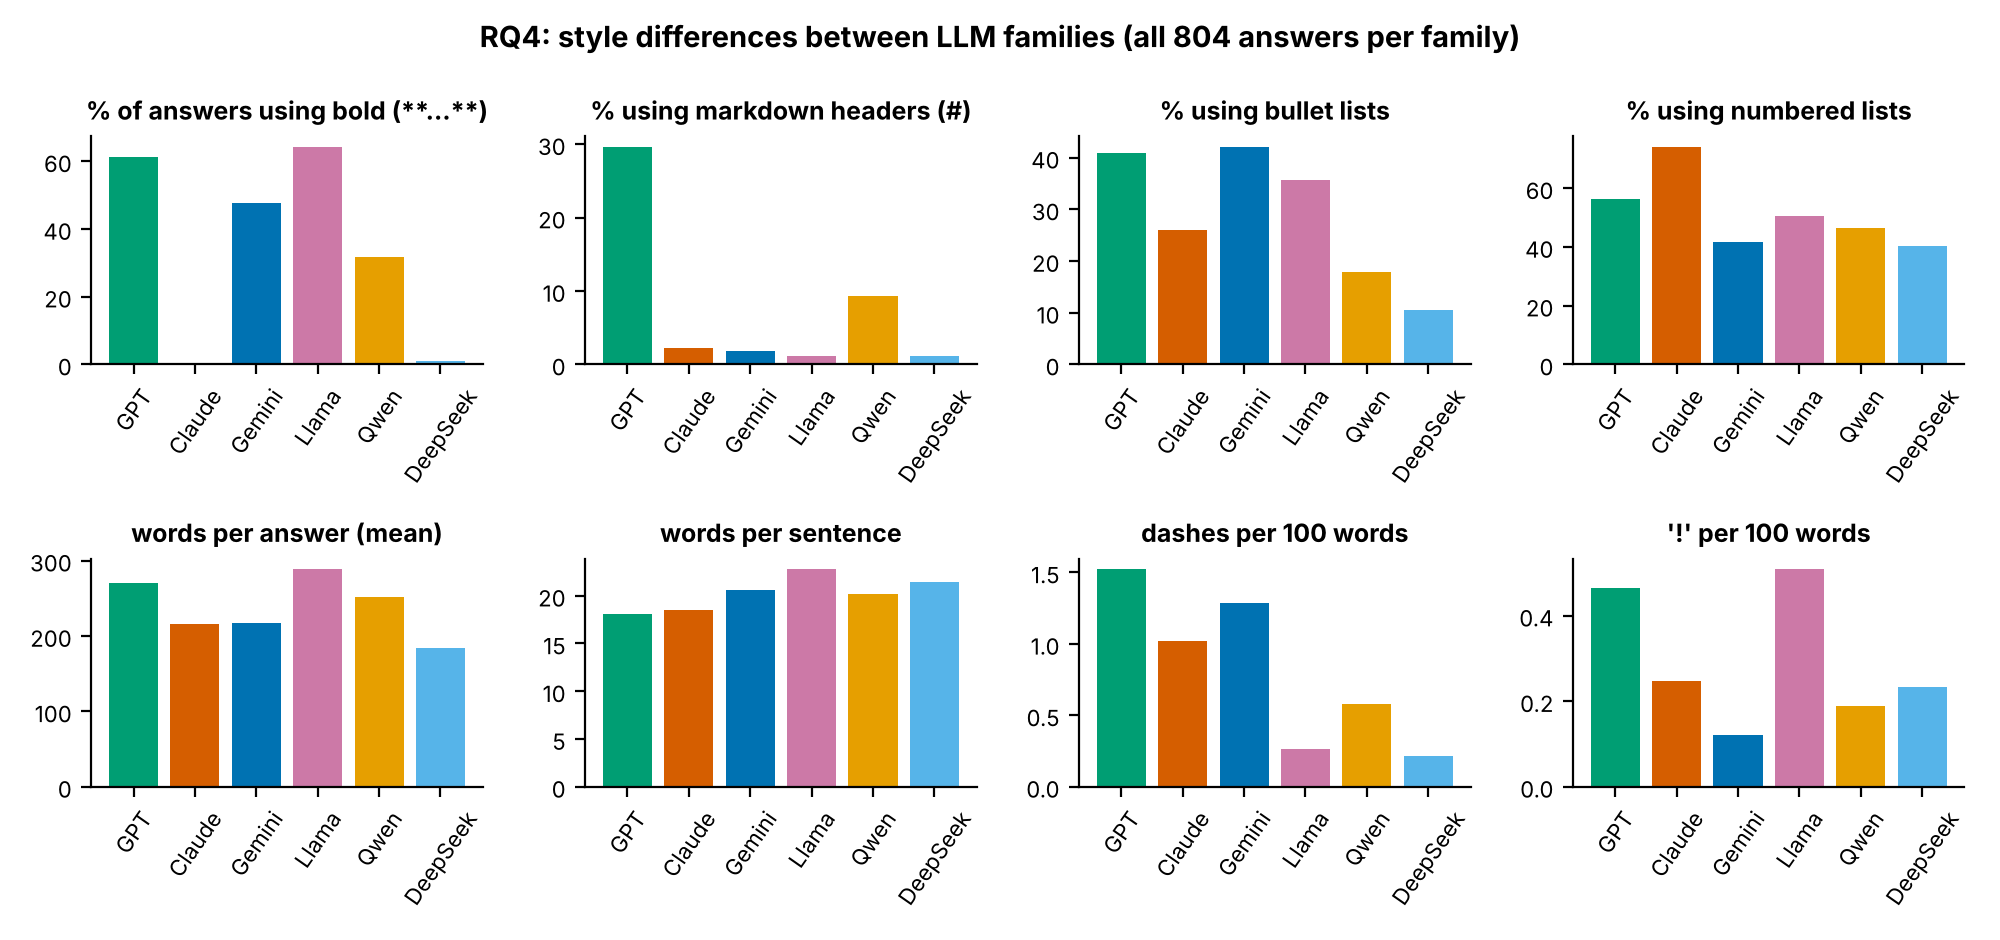
\includegraphics[width=0.98\linewidth]{fig_rq4_style.png}
\caption{Style differences between the LLMs. Top row: \% of answers that use each kind of formatting at least once.
Bottom row: averages.}
\label{fig:style}
\end{figure}

Some small habits work almost like a signature (Table~\ref{tab:markers}). GPT uses the curly apostrophe
(\textquoteright) in \CurlyGpt\% of its answers, and only Qwen also does (\CurlyQwen\%). Llama writes bullets with
\texttt{*} and is the only one that opens with ``What a great question!''. Claude and Llama often start with
``Here's'', and GPT with ``Sure'' or ``Certainly''.

\begin{table}[!htbp]
\centering
\caption{Signature habits: \% of each LLM's answers that show the habit.}
\label{tab:markers}
\small
\begin{tabular}{lrrrrrr}
\toprule
Habit & GPT & Claude & Gemini & Llama & Qwen & DeepSeek \\
\midrule
\tabinput{tables/rq4_markers.tex}
\bottomrule
\end{tabular}
\end{table}

\textbf{What do the classifiers look at?} The TF-IDF model's strongest features are mostly formatting marks
(\ttt{**}, \ttt{\#\#\#}, a line break before a list) and typical phrases (``sure!'', ``here's a'', ``what a'',
``therefore''). I also looked at the pieces of text that switch on the CNN's strongest filters, and they match the
same habits: ``\#\#\# step'' headers for GPT, ``here's why:'' for Claude, ``what a great question!'' for Llama and
``therefore,'' for Gemini. A logistic regression that sees only 22 simple style numbers gets \FeatAllFeatures\%.
The 7 formatting numbers alone give \FeatFormattingOnly\%, more than the 12 wording numbers, such as sentence
length and punctuation (\FeatLinguisticOnly\%), or the 3 length numbers (\FeatLengthOnly\%).

\textbf{Removing one kind of signal.} Finally, I changed the answers in five ways (Table~\ref{tab:ablation}) and
tested the CNN in two ways. First, the normal CNN is tested on the changed answers: this shows how much it
\emph{relies} on what I removed. Second, a new CNN is trained on the changed answers: this shows whether
\emph{enough other information is left} to recognize the LLM.

\begin{table}[!htbp]
\centering
\caption{RQ4: CNN test accuracy (\%) after removing one kind of signal (average of 3 seeds).}
\label{tab:ablation}
\small
\begin{tabular}{lcc}
\toprule
What the CNN sees & \two{Normal CNN, tested}{on changed answers} & \two{New CNN, trained}{on changed answers} \\
\midrule
The full answer (nothing removed) & \AblOriginalTest & \AblOriginalRetrain \\
No markdown and no line breaks & \AblNoFormatTest & \AblNoFormatRetrain \\
Words only (no punctuation or formatting) & \AblWordsOnlyTest & \AblWordsOnlyRetrain \\
Structure only (every word replaced by \ttt{<w>}) & \AblStructureOnlyTest & \AblStructureOnlyRetrain \\
First 30 tokens only & \AblOpeningOnlyTest & \AblOpeningOnlyRetrain \\
A middle piece only (tokens 50--150) & \AblMiddleOnlyTest & \AblMiddleOnlyRetrain \\
\bottomrule
\end{tabular}
\end{table}

\textbf{(i) What does the classifier use? Mostly the structure of the answer.} When every word is replaced by the
same placeholder, so the CNN only sees punctuation, line breaks and markdown, a new CNN still gets
\AblStructureOnlyRetrain\%, close to the \AblOriginalRetrain\% for the full answer. With only the words, it gets
\AblWordsOnlyRetrain\%.

\textbf{(ii) Words or structure? Both, but structure is stronger.} Words alone are still far above guessing, so
word choice (``here's'', ``certainly'', ``therefore'') carries real signal. The shape of the answer carries more.

\textbf{(iii) Does removing these signals hurt? Yes, a lot.} Without markdown and line breaks, the normal CNN drops
from \AblOriginalTest\% to \AblNoFormatTest\%. A new CNN trained without them gets some of it back
(\AblNoFormatRetrain\%), but not all. The fingerprint is also spread over the whole answer: the first 30 tokens
give \AblOpeningOnlyRetrain\%, and a piece from the middle gives \AblMiddleOnlyRetrain\%. So just asking an LLM to
answer in plain text, without markdown, would already hide much of its identity.

\section{Lessons and experience}

\textbf{1. The dataset design decides what you can conclude.} Because all six LLMs answered the same prompts, the
prompt-only test lands exactly on chance, and the topic of a prompt cannot sneak into my RQ1 numbers. My
simulation showed how a biased collection could create a fake fingerprint: \BiasOneLr\% accuracy from prompts
alone. Now, when I see a high accuracy, my first question is: what else could the model be using?

\textbf{2. How you split the data matters.} I split by prompt. Later I tried a random split by row: TF-IDF fell
from \LrAcc\% to \RowSplitLr\%. With a row split, the other five answers to a test prompt sit in the training data
under other labels, and their shared topic words point to the wrong LLM. The split changed my result by about
\RowSplitGap{} points.

\textbf{3. Start with a simple baseline.} TF-IDF + logistic regression trained in seconds and was as good as my
neural classifiers. The BiLSTM was about 5 times slower and a bit worse. With only about 3,400 training answers,
a deep model does not win automatically.

\textbf{4. Preprocessing is a modeling choice.} I kept line breaks and markdown as tokens because I guessed that
formatting mattered, and RQ4 showed it is the strongest signal. The usual ``lowercase and remove punctuation''
step would have thrown much of it away.

\textbf{5. Check labels made by rules.} My keyword rules put ``Write a script for a YouTube video'' under coding.
Reading the coding and math prompts by hand found 38 wrong labels, and RQ3 depends on these labels.

\textbf{6. Plan around your computer, and report the spread.} I had no GPU, so I timed one epoch before planning
anything. My first BiLSTM needed about 5 minutes per epoch, so I made it smaller and cut the answers to 250
tokens. I also learned that one run is not enough: the same CNN got anywhere from \CnnMin\% to \CnnMax\%
depending on the random seed.

\section{Limitations}

\begin{itemize}
  \item \textbf{One model per family.} The classifier learns these six models, not whole families. The models are
        also from different years (Gemini Pro and DeepSeek-LLM-67B are from 2023, the others from 2024), so some
        differences may come from model age.
  \item \textbf{Default settings only.} All answers come from AlpacaEval's standard setup. A user who asks for
        ``no markdown'' could hide much of the fingerprint.
  \item \textbf{Small test set.} The test set has 732 answers, so differences of 2--3 points can be noise.
  \item \textbf{Not proof.} About 1 in 3 answers is still labeled wrong, so a tool like this must never be used as
        proof of who (or what) wrote a text.
\end{itemize}

\textbf{How to reproduce.} The code, the dataset, all results and the training logs are at
\url{https://github.com/borispie/who-wrote-it-llm-id}. Run \ttt{pip install -r requirements.txt} and then
\ttt{bash run\_all.sh} (about 4--5 hours on a 2-core CPU). The README explains each step.

\begin{thebibliography}{9}
\bibitem{alpacaeval} X. Li, T. Zhang, Y. Dubois, R. Taori, I. Gulrajani, C. Guestrin, P. Liang, T. B. Hashimoto.
  \emph{AlpacaEval: An Automatic Evaluator of Instruction-following Models.} GitHub repository
  \ttt{tatsu-lab/alpaca\_eval}, 2023.
\bibitem{kim2014} Y. Kim. Convolutional Neural Networks for Sentence Classification. \emph{EMNLP}, 2014.
\bibitem{lstm} S. Hochreiter and J. Schmidhuber. Long Short-Term Memory. \emph{Neural Computation}, 9(8), 1997.
\bibitem{adamw} I. Loshchilov and F. Hutter. Decoupled Weight Decay Regularization. \emph{ICLR}, 2019.
\bibitem{mattr} M. A. Covington and J. D. McFall. Cutting the Gordian Knot: The Moving-Average Type-Token Ratio
  (MATTR). \emph{Journal of Quantitative Linguistics}, 17(2), 2010.
\end{thebibliography}

\end{document}
